\documentclass[a4paper,10pt]{article}

%\usepackage{natbib}
\usepackage{amsthm}
\usepackage{amsfonts}
\usepackage{amssymb}
\usepackage{amsmath}
\usepackage{latexsym}
\usepackage{graphicx}
\usepackage{blindtext}

\usepackage{doc}

\newtheorem*{theorem}{Theorem}
\theoremstyle{definition}
\newtheorem*{definition}{Příklad}


\hoffset -1in \topmargin 0mm \voffset 0mm \headheight 0mm
\headsep0mm
\oddsidemargin  20mm     %   Left margin on odd-numbered pages.
\evensidemargin 20mm     %   Left margin on even-numbered pages.
\textwidth   170mm       %   Width of text line.
\textheight  252mm

\makeatletter
\renewcommand\@openbib@code{%
     \advance\leftmargin  \z@ %\bibindent
      \itemindent \z@
     % Move bibitems close together
     \parsep -0.8ex
     }
\makeatother

\makeatletter
\renewcommand\section{\@startsection {section}{1}{\z@}%
                                   {-3.5ex \@plus -1ex \@minus -.2ex}%
                                   {1.5ex \@plus.2ex}%
                                   {\large\bfseries}}
\makeatother

\makeatletter
\renewcommand\subsection{\@startsection {subsection}{1}{\z@}%
                                   {-3.5ex \@plus -1ex \@minus -.2ex}%
                                   {1.5ex \@plus.2ex}%
                                   {\normalsize\bfseries}}
\makeatother

\makeatletter
	\setlength{\abovecaptionskip}{3pt}   % 0.25cm 
	\setlength{\belowcaptionskip}{3pt}   % 0.25cm 
\makeatother

\usepackage[utf8]{inputenc}
\usepackage{array,pifont,xcolor}
\newcommand{\fajfka}{\textcolor[RGB]{0,166,79}{\ding{51}}}
\newcommand{\krizek}{\textcolor[RGB]{237,27,35}{\ding{55}}}

\begin{document}
\pagestyle{empty}

\renewcommand{\figurename}{Obr.}
\renewcommand{\tablename}{Tab.}

\begin{center}
{\bf \Large Chatboti}
\end{center}

\smallskip
\begin{center}
{\large Anna Kučerová}
\end{center}

\smallskip
\begin{center}
Faculty of Mechanical Engineering, Brno University of Technology\\
Institute of Automation and Computer Science\\
Technicka 2896/2, Brno 616 69, Czech Republic\\
Name.Surname@vutbr.cz\\
\end{center}

\bigskip
\noindent Abstrakt: \textit{Tato práce se zaměřuje na chatboty, jejich vývoj, architekturu a využití. Dále obsahuje popis některých základních principů, které se při konstrukci chatbotů využívají.}

\vspace*{10pt} \noindent Klíčová slova: \textit{Chatbot, Loeberova cena, ALICE, AIML, Mitsuku, Cleverbot, ChatScript, Watson, Siri}

\bigskip
\section{Úvod}
\label{sec:1}

Chatbot je program navržený pro chytrou komunikaci s lidmi ať už pomocí textu nebo mluveným slovem. Jeho cílem je vyvolat pocit, že si píšete, či mluvíte, se skutečným člověkem. V dnešní době se s chatboty setkáváme stále častěji ve formě chatovacího okénka na sociálních sítích a e-shopech, nebo aplikace v mobilu či autě ovládané hlasem. Cílem chatbota je napodobit, co nejpřesněji mezilidskou komunikaci. 

\section{Vývoj}
\label{sec:2}

I když se zdá, že chatboti jsou poměrně moderním vynálezem, prvním chatbot, který dokázal napodobit člověka (i když ne na takové úrovni, jak je tomu dnes), byl naprogramovaný už v roce 1966 a nesl jméno ELIZA. Princip ELIZY spočíval v identifikaci klíčových slov vstupní věty a pomocí vzorových shod s před programovanými pravidly by vygenerovala odpověď.

V pořadí dalším známějším chatbotem byl bot jménem PARRY. Byl vytvořen v roce 1972 a napodoboval paranoidního schizofrenika.
Více komplexním a velmi známým chatbotem je ALICE. Ten uměl odpovídat na základě vzorů přiřazených vstupu (tedy tomu, co mu napíše uživatel) ke dvojicím uložených v databázi, která byla generována umělou inteligencí. Svou slávu si získala třemi výhrami Loebnerovy ceny.

V současné době se setkáváme s velmi chytrými chatboty, kteří nejen že odpovídají na otázky, ale zvládají plnit i jednoduché příkazy: přesměrování na stránku s hledaným produktem (Ikea: Anna), vytočit telefonní číslo nebo třeba najít předpověď počasí (Apple: Siri, Microsoft: Cortana, Mercedes-Benz: Mercedes atd…). Kromě chatbotů, které firmy využívají, jako své maskoty ukazující jejich prestiž, se v poslední době začínají rozvíjet osobní pomocníci, či chatovací "doktoři" (terapeutický chatbot: Woebot, plánovač dovolené: Wayblazer, správce financí: Financial Advisor). Mezi nejlepší lidské společníky patří Mitsuku bot, který od roku 2005 zvládl pětkrát vyhrát Loebnerovu cenu. 



\section{Loebnerova cena}
\label{sec:2}

V předešlém textu byla naznačena jistá prestiž Loebnerovy ceny. Jedná se o soutěž umělé inteligence založenou v roce 1990, která je postavena Turingově testu. Na jedné straně je porotce, který zároveň komunikuje s jiným člověkem a chatbotem, aniž by předem věděl, kdo je kdo. Z této komunikace se snaží určit, který z respondentů je člověk a který program. Autoři robotů využívají různých technik, které jim mohou dopomoci k vítězství. Patří mezi ně záměrné psaní hrubek a překlepů, naprogramování minulosti robota, aby zvládl vzpomínat na dětství a mnohá další. Jakmile bude naprogramovaná umělá inteligence, které zvládne Turingův test, soutěž bude ukončena.

\begin{table}[h] 
\begin{center}
\label{tab:1}
\begin{tabular}{llllll}
\hline\noalign{\smallskip}
& Expertní systém: & Analytická AI & Lidmi inspirovaná AI & Polidštěná AI & Člověk\\
\hline Kognitivní iteligence & \krizek & \fajfka & \fajfka & \fajfka & \fajfka \\
Emoční inteligence & \krizek & \krizek & \fajfka & \fajfka & \fajfka \\
Sociální inteligence & \krizek & \krizek & \krizek & \fajfka & \fajfka \\
Umělecká inteligence & \krizek & \krizek & \krizek & \krizek & \fajfka \\
\hline
\end{tabular}
\caption{Srovnání umělých inteligencí s člověkem} 
\end{center}
\end{table}

Roboti jsou zkoušeni v jednotlivých inteligenční kategoriích (kognitivní inteligence, sociální inteligence, emocionální inteligence a kreativita.) První tři kategorie jsou již dosažené. Problém obvykle nastává v umělecké inteligenci. Aby robot zvládl Turingův test, musí dokázat zpracovat informace ze zvuku a obrazu. A to ne jenom po informační stránce ale také po stránce emoční. \cite{5}\cite{c}

\section{Návrh jednoduchého chatbota}
\label{sec:3}
Kromě volby operačního systému, programovacího jazyka nebo tvorby chatovacího okna je nutné implementování přiřazování vzorů. Vstupní text se přiřadí k hodnotám, které jsou uloženy v databázi a odpovídají vstupu. Pomocí tohoto jednoduchého postupu je chatbot schopen komunikovat s člověkem za pomocí jednoduchých, zřetelných vět. 

Nezbytnou nutností je implementace databáze, kterou chatbot využívá. Databáze je tvořena dvourozměrným polem, jehož sudé řádky obsahují požadavky/otázky a liché řádky příslušné odpovědi. Na prvním řádku se zpravidla uvádějí odpovědi, které bot použije nedojde-li ke shodě. Řádek obsahuje pouze jeden typ požadavku/otázek nebo odpovědi.

\begin{figure}[h] 
\begin{center}
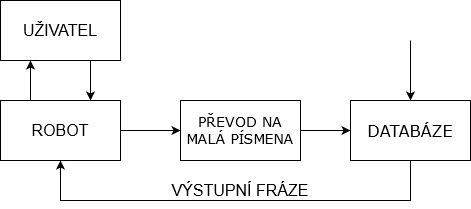
\includegraphics[scale=0.4]{image/2.jpg}
\caption{Schéma chatbota}
\label{fig:1}
\end{center}
\end{figure}

\begin{definition}
Je-li na řádku A otázka: "Jak se máš?", může zároveň obsahovat otázku: "Jak je?".
Naproti tomu, řádek B bude obsahovat n odpovědí typu: "Mám se dobře.", "Je mi dobře." a tomu odpovídajících variant.
\end{definition}


Hledání shody probíhá následovně: uživatelský vstup se převede na malá písmena a nastaví se proměnná response na nulu. Pokud dojde ke shodě, hodnota response zůstane na nule a vrátí možný výstup, pokud nedojde, response se nastaví na hodnotu jedna a vrátí možnou variantu nastavenou na prvním řádku databáze (odpovědi pro případ, že nenastane shoda). \cite{7}\cite{4}

\section{ALICE}
\label{sec:4}

Jak již bylo zmíněno, bot ALICE ("Artificial Linguistic Internet Computer Entity" tedy: "umělá jazyková internetová počítačová entita") je trojnásobnou výherkyní Loebnerovy ceny. Přes své úspěchy však nezvládne projít Turingovým testem. Rozpoznatelnost od člověka je zcala patrná z tabulky (Tab.~2), vlevo, který je záznamem komunikace ALICE s uživatelem ve volně dostupné internetové aplikaci.\cite{3}\cite{a}

\begin{table}[h] 
\begin{center}

\label{tab:1}
\begin{tabular}{llll}
\hline\noalign{\smallskip}
Uživatel: & May I have a question? & Uživatel: & May I have a question? \\
A.L.I.C.E:& Not right now, maybe later.      & Kuki\_ai: & Why doesn't Tarzan have a beard? \\
&&&\\
Uživatel: & But. I’m sad. & Uživatel: & No, I‘m sad.\\
A.L.I.C.E:& And. What makes you so sad, ANNA.      & Kuki\_ai: & That was not a yes or no question. \\
&&&What are you sad about Ann?\\
&&&\\
Uživatel: & I lost my job. & Uživatel: &I lost my job. \\
A.L.I.C.E:&Where did you last see it.     & Kuki\_ai: & I am sorry to hear it.\\
&&& A lot of people are unemployed now. \\
\hline
\end{tabular}
\caption{Rozhovor uživatele s ALICí a pro porovnání obdobný rozhovor s Mitsuki } 
\end{center}
\end{table}

\subsection{AIML}
\label{subsec:1}

AIML je umělá inteligence, kterou má mimo jiné implementovanou ALICE. Základní jednotkou jsou kategorie, které obsahují vstup (pattern) a výstup (template). Vstup je otázka nebo uživatele, výstup je reakce umělé inteligence na vstup. Každý soubor AIML začíná nastavením použité verze. 
Umělá inteligence AIML má implementovanou rekurzi \textless srai\textgreater\ díky které je schopná hledat vzor opakovaně dokud jej nenajde. Toto se může hodit v případě, že použijeme jednu z možných n frází, které mají stejný význam ("mám dvacet let", "je mi dvacet", "můj věk je dvacet"…), pokud uživatel udělá pravopisnou chybu, či překlep při zadávání vstupu nebo například při delších větách, které rozdělí na více častí, a tak může hledat kategorii pomocí více vzorů. \cite{8}\cite{5}\cite{b}

Kontextová část se skládá ze dvou parametrů \textless that\textgreater\ a \textless tpic\textgreater. Značka \textless that\textgreater\ se musí shodovat s posledním výrokem robota, především v případě, že položí otázku. Vyskytuje se uvnitř kategorie. Naproti tomu \textless topic\textgreater\ se vyskytuje vně kategorie a shromažďuje je dohromady. V tabulce (Tab.~3) je zapsána ukázka kódu. Uživatel zasílá ALICI zprávu a ta na ni reaguje.


\begin{table}[h] 
\begin{center}

\label{tab:1}
\begin{tabular}{l}
\hline\noalign{\smallskip}
\textless aiml version =‘‘1.01‘‘\textgreater\\
\textless category\textgreater\\
\textless pattern\textgreater\ I lost my job \textless /pattern\textgreater\\
\textless template\textgreater\\
\textless srai\textgreater\ Where did you last see it. \textless star\ \textgreater\ \textless /srai\textgreater\\
\textless /template\textgreater\\
\textless /category\textgreater \\
\textless /aiml\textgreater\\
\hline
\end{tabular}
\caption{Ukázka AIML kódu} 
\end{center}
\end{table}

\section{Současnost}
\label{sec:5}

Dnešní chatboti jsou uživatelsky přístupnější, než tomu bylo v minulosti. Mnozí z nich se rozvinuli od pouhého textového povídání do hlasových asistentů. Snaží se být vtipní, empatičtí, dostávají přízvuky a tváře. Uživatel si s nimi může povídat, hrát hry, dávat jim úkoly, které zvládají plnit napojením do systému atd. Jejich cílem je pobavit a ulehčit uživateli práci.
Také jejich struktura je propracovanější. Mnozí upustili od AIML, přidali heuristické algoritmy, strojové učení a mnoho dalšího. \cite{1}

\subsection{Mitsuku}
\label{subsec:1}


Poslední a pětinásobný výherce Loebnerovy ceny má také jako ALICE implementovanou AIML, avšak pro hledání shody používá heuristických algoritmů. Databázi svých znalostí rozšiřuje pomocí strojového učení pod dohledem, takže pokud se dozví něco nového, odešle data ke schválení a po autorizaci je začlení do databáze. Kromě konverzačních schopností je zapracován do sítě (facebook, twiter), kde vystupuje pod jménem Kuki\_ai a vytváří dojem skutečné osoby. Při konverzaci si pamatuje údaje o uživateli, a dokonce zvládá uvažovat o objektech. Zeptáte-li se ho: "Můžu jíst dům?", vyhledá údaje o domě, zjistí že je z cihel a odpoví: "Ne." Ne vždy je ale jeho odpověď správná. Pokud se jej zeptáte, jestli může jíst stromy, najde v databázi, že strom je rostlina a podle jeho pravidel, lidé můžou jíst rostliny. Takovéto i mnohem delší rozhovory zvládá v padesáti šesti jazycích. V tabulce (Tab.~2) je ukázka rozhovoru pro srovnání s ALICí.

\subsection{Cleverbot}
\label{subsec:2}

Cleverbot je oblíbený zábavný chatbot. Data shromažďuje online, při komunikaci s lidmi. Na rozdíl od jiných chatbotů neodpovídá Cleverbot podle předem naprogramovaných odpovědí, ale simuluje spontánní konverzaci. Nejdříve uživatel zadá vstup bot vyhledá všechna klíčová slova odpovídající zadání. Výstup vybere podle předešlých reakcí uživatelů v minulosti. Cleverbot má stejně jako Kuki ai svého avatara.

\subsection{ChatScript}
\label{subsec:3}

Oproti předešlým robotů. ChatScript nevyužívá AIML, ale kombinaci systému pro správu dialogu a stroje přirozeného jazyka. Pravidlo se skládá ze štítku, typu, vzoru a výstupu. Jednotlivá pravidla se seskupují do tzv. témat. ChatScrip najde shodu tématu a poté používá pravidlo, které je v tématu obsaženo. Díky tomuto je vhodný pro aplikace jako jsou "help desk", informační systémy atd. 

\subsection{Watson}
\label{subsec:4}

Velice zajímavým chatbotem s neskutečně velkou škálou možností využití, díky schopnosti práce s velkým objemem dat, je chatbot Watson. Získávání informací a zodpovězení otázek provádí pomocí kombinace zpracování přirozeného jazyka a metodu hierarchického strojového učení. Ke generování odpovědí používá širokou škálu mechanismů k identifikaci a přiřazení hodnot funkcí, jako jsou jména, data atd. Systém strojového učení se pak učí, jak kombinovat hodnoty těchto funkcí do konečného skóre pro každou odpověď. Na základě tohoto skóre se všechny možné odpovědi seřadí a vybere nejlepší. 

\subsection{Siri}
\label{subsec:5}

Nelze nezmínit hlasovou asistentku Siri od firmy Apple poprvé připojenou v roce 2010. Ačkoli zprvu zvládala pouze rozpoznání hlasů, dnes je už o mnoho úrovní výše. Na požádání vypráví vtipy, vytáčí hovory, hledá informace na internetu a mnoho dalšího. Asistentka se s rostoucím využitím přizpůsobuje svému uživateli (jazykovým zvyklostem, preferencím ve vyhledávání na internetu atd.). \cite{c}

Jako reakci na hlasovou asistentku firmy Apple, vyvinula a v roce 2014 představila společnost Microsoft vlastní aplikaci s názvem Cortana, může ji najít mimo jiné na Xboxu. A v roce 2016 přišel se svou hlasovou asistentkou Google, používanou pro platformu Android.

\section{Závěr}
Od nejstaršíhu chatbota se jejich kvalita posunula velmi významě dopředu. V dnešní době zvládají mnohem víc číností, než zpočátku. Rozšířili se skrze platformy a díky jednoduchosti používání významě rostou na oblibě. Jejich praktičnost a široká škála možného využití vytváří motivaci v jejich pokračování a zdokonalování a snahu vytvořit umělou inteligenci, která bude k nerozeznání od lidské.\cite{6}\cite{2}



% References
%
\begingroup
\makeatletter
\renewcommand\section{\@startsection {section}{1}{\z@}%
                                   {-3.5ex \@plus -1ex \@minus -.2ex}%
                                   {4.5ex \@plus.2ex}%
                                   {\large\bfseries}}
\makeatother

\renewcommand{\refname}{Reference}

\bibliography{references}{}
\bibliographystyle{acm}
\endgroup

\end{document}